\documentclass[letterpaper,11pt,oneside]{article}
%\documentclass[a4paper,11pt,oneside]{article}

% J. Bioinformatics  see
%   http://www3.oup.co.uk/jnls/list/bioinformatics/instauth/
%   LATEX article style format, two-column text with 86mm columns
%   Figures either one-col (86mm) or double (178 mm) wide.
%   References must NOT be numbered,
%   listed in *alphabetical* order:
%   surname, initials, (year), paper title, journal, volume, pp. pages

\usepackage{multicol}

\usepackage{times}
%\usepackage{epsfig}

\usepackage{verbatim}

\usepackage{bioinformatics}

\usepackage[none,bottom,dark,english]{draftcopy}
\draftcopyName{ DRAFT \number\day\/\number\month\/\number\year}

\usepackage[verbose]{geometry}
\geometry{top=2cm,bottom=2cm,left=14mm,right=14mm,nohead}

\setlength{\columnsep}{10mm}

%\geometry{top=1in,bottom=1in,left=1in,right=1in,nohead}

\def\plotwidth{0.75\columnwidth}

%\setlength{\parindent}{0pt}
%\setlength{\parskip}{1.0ex plus0.5ex minus0.5ex}


%Check if we are compiling under latex or pdflatex
\ifx\pdftexversion\undefined
  \usepackage[dvips]{graphics}
\else
  \usepackage[pdftex]{graphics}
\fi



\begin{document}

\title{ Modelling-Alignment for Sequences of Mixed or
of Medium to Low Information-Content }
% ?models don't shuffle?  ha, ha

\author{
  David R. Powell\footnotemark[1]~\footnotemark[2]~~$^{1,2}$, Lloyd Allison$^2$ and Trevor I. Dix$^{1,2}$ \\
  $^1$Victorian Bioinformatics Consortium and \\
  $^2$School of Computer Science and Software Engineering, \\
  Monash University, Australia 3800.
}

\renewcommand{\thefootnote}{\fnsymbol{footnote}}
\footnotetext[1]{To whom correspondence should be addressed.}
\footnotetext[2]{Partially funded by Australian Research Council Grant A49800558.}
\renewcommand{\thefootnote}{\arabic{footnote}}

\date{}
\maketitle

%-------------------------------------------------------------------------

\begin{multicols}{2}

%\toappear{Submitted to ? J. Bioinformatics ? 2002.}

\begin{abstract}

\noindent
{\bf Motivation:}
Populations of biased, non-random sequences may cause standard alignment
algorithms to yield false-positive matches and false-negative misses.
A standard significance test based on the {\em shuffling} of
sequences is a partial solution, applicable to populations that can
be described by {\em simple} models.
Masking-out low information content intervals throws information away.
We describe a new and general method, {\em modelling-alignment}:
Population models are incorporated into the alignment process,
which can (and should) lead to changes in the rank-order of matches
between a query sequence and a collection of sequences,
compared to results from standard algorithms.
The new method is general and places very few conditions on
the nature of the models that can be used with it.
We apply modelling-alignment to local alignment, global alignment,
optimal alignment, and the relatedness problem.

\noindent
{\bf Results:}
As expected, modelling-alignment and the standard {\tt prss} program from
the FASTA package have similar accuracy on sequence populations that
can be described by simple models, e.g. 0-order Markov models.
However, modelling-alignment has higher accuracy on populations
that are {\em mixed} or that are described by higher-order models:
It gives fewer false positives and false negatives as shown by
ROC curves and other results from tests on
real and artificial data.

\noindent
{\bf Availability:}
An implementation of the software is available via the
Web~\footnote{http://www.csse.monash.edu.au/$\sim$powell/m-align.tar.gz}.

\noindent
{\bf Contact:}
powell@csse.monash.edu.au

%\noindent
%Supplementary Information:
%t.b.a..

\end{abstract}


%-------------------------------------------------------------------------
\section{Introduction} \label{sec:Intro}

Alignment algorithms are used to answer two quite different kinds of questions,
(i) Are two (or more) sequences {\em related} or not?
(ii) {\em How} are two (or more) sequences related,
{\em given} that they are related?
There is a ``fundamental difference between
the searching [for related sequences] and [optimal] alignment operations.'' --
\cite{gribskov96}.
It is also well known that populations of biased, non-random,
low information content sequences may cause algorithms
to return false-positive matches and false-negative misses for
the first kind of problem and may also cause poor alignments,
for the second kind of problem.
There are partial solutions, with disadvantages:
Masking-out low information content intervals~\cite{claverie93}
can reduce false-positives but it throws away some information and
raises the question of how low is low.
The significance of a possible match is often assessed by comparing
its score (or cost) with those obtained when ``one member of
the protein [say] pair [is] randomized"
(shuffled, permuted) -- \cite{needleman70}.
We call this general kind of significance testing {\em shuffling};
note that an alignment is calculated under the assumption of random sequences
and {\em then} the shuffling test is applied, possibly to a bad alignment
if the sequences are non-random.

We describe a new method, {\em modelling-alignment} (M-alignment)
which incorporates explicit models of sequence populations.
It is based on the premise that two sequences are related if one tells
something {\em new} and {\em useful} about the other,
i.e. something not otherwise known.
It has a natural null-theory and hypothesis test.
Instead of a low information interval being masked-out, it is given
a low, but non-zero, weight thus not discarding information.

A high information interval, i.e. a {\em feature}, is given a high weight;
there is a big scoring advantage if it is matched in another sequence.
In general this can, and should, change the rank-order of alignments
between two sequences and the rank-order of matches between multiple sequences.
There is no hard (and arbitrary) threshold for what is
a {\em background} low information interval or
for what is a high information feature;
there is a continuous spectrum of information content from low to high.

M-alignment is general and places few restrictions on the kind
of population model that can be used with it.
If the ``correct'' model is not known in advance
there are some sensible candidates to try
and a good model can be detected on the basis of information content.
Algorithm time-complexity remains $O(n^2)$ for reasonable models.
This paper extends work on the 1-state mutation model~\cite{allison99}
by applying M-alignment to
the relatedness and optimal alignment problems,
for both global \cite{needleman70} and local \cite{smith81} alignment,
under the 3-state, affine gap-costs model \cite{gotoh82} of mutation.

M-alignment results are compared to those of
the {\tt prss} program -- from the FASTA package~\cite{pearson96} -- which
is based on {\tt rdf2}~\cite{pearson88} with a shuffling significance test.
Receiver operating characteristics (ROC) curves show that, as expected,
both methods give similar results
on simple data, i.e. uniform and 0-order Markov model populations.
M-alignment is more accurate,
i.e. gives fewer false positives and fewer false negatives,
on mixed populations,
on populations of mixed sequences, and
on populations described by higher-order models.

At this point it is convenient to clarify some of the terminology we use in
this paper.  We use the term {\em rank-order} to mean order obtained when
items are ranked according to some score.  When a group or population of
sequences is well explained by a particular model, we say that model is a
{\em population model} for those sequences.  An alignment can be seen as a
hypothesis of how two (or more) sequences are related.  Using
information-theoretic techniques we can quantify how likely a hypothesis is,
and thus discuss the {\em probability of an alignment}.

%-------------------------------------------------------------------------
\section{Systems and Methods} \label{sec:sys}

\subsection{Models} \label{sec:models}
% non-random, compress'n, inf'n, seq' models, Markov m', Bayes, MML...

There is considerable interest in the compression of biological
sequences~\cite{grumbach94,loewenstern96,rivals97,allison00},
not so much to save disc space but
as a criterion for comparing models of populations of sequences.
The terms {\em biased}, {\em non-random}, {\em low information content}
and {\em compressible} are equivalent for our purposes:
If DNA bases, say, are generated uniformly at random, an optimal code
assigns each one a two-bit code.
This follows from
Shannon's mathematical theory of communication~\cite{shannon49}.
If the DNA comes from a biased 0-order model say,
shorter codes can be allocated {\em on average}.
For example, if the respective probabilities of an A, T, G or C are [1/2, 1/4,
1/8, 1/8] this leads to optimal codes of
[1, 2, 3, 3]-bits respectively, that is 1~3/4-bits on average.
For higher-order models, code-words depend on the {\em context}
of previous characters, on the `k' previous characters
for a Markov model of order~k.
Probabilistic finite-state automata (PFSAs),
also known as hidden Markov models,
have been used as models~\cite{georgeff84} of populations of sequences.
Each of these models, and many others, can deliver a probabilistic
prediction for the next character in a sequence given a context.
From Shannon, the length of a code-word for the next character,
its {\em message length}, is the -log of this probability and
is a measure of the information content of the character in the context.
M-alignment uses this quantity.


\subsection{Relatedness and Alignment} \label{sec:rel}
% if v. how

The generic dynamic programming algorithm (DPA) for
sequence comparison can be used to find various kinds
of global alignments depending on how it is instantiated: E.g.
Given {\em scores} of one for a match and zero for mismatch, insert and delete,
the DPA finds the longest common subsequence (LCS).
Given {\em costs} of zero for a match and one for mismatch, insert and delete,
it finds an optimal alignment under the Levenshtein~\cite{levenshtein66}
metric also known as the simple
edit-distance~\cite{sellers74}.
{\em Affine} gap-costs, for runs of inserts or deletes,
are more plausible biologically and Gotoh~\cite{gotoh82}
gave such an alignment algorithm; the key is to have three {\em states}
for each cell in the DPA's matrix, for costs (or scores)
{\em conditional} on diagonal, vertical and horizontal moves.

All of the above DPA variations find a global optimal alignment for
some given criterion, or at least under the assumption that,
two sequences are related.
Shuffling tries to solve the relatedness problem by comparing the
score (or cost) of an optimal alignment with the scores (costs)
of alignments of the randomized sequences.
If the former is not significantly better than the latter
the sequences are deemed to be unrelated.
The idea is that randomized sequences are {\em like} their originals in
general statistical terms but are otherwise unrelated.
Shuffling preserves 0-order statistics of sequences.
It can be arranged to preserve 1st-order statistics~\cite{fitch83}
and even codon usage~\cite{altschul85} but it is hard to imagine how
to carry it out while preserving the statistics of an arbitrary model
particularly if that is a mixture or is high-order.

A different approach to the relatedness problem
considers a probabilistic {\em mutation model}.
The costs (scores) of the DPA are replaced by the -log probabilities
of match, mismatch, insert and delete.
In fact costs and scores can be {\em normalized}~\cite{allison93a} to show
the underlying probabilities.
The DPA can then find a {\em most probable} alignment, but it can also
be modified to calculate the {\em joint} probability of two sequences:

\begin{minipage}{0.9\columnwidth}
An alignment is just a hypothesis.
The set of all alignments is exclusive and exhaustive, given that
two sequences are related.
Rather than selecting the largest probability,
their probabilities can therefore be {\em added}.
\vspace{0.5em}
\end{minipage}
\noindent
This was originally done for a 1-state mutation model \cite{bishop86}.
Later, it was extended \cite{allison92a} to 3-state (linear gap-costs)
and 5-state (piece-wise linear gap-costs) mutation models,
and included the cost (complexity) of models so that simple
and complex models can be compared fairly.
Such considerations also give
a natural {\em null-theory} that the sequences are not related,
i.e. that one tells nothing new or useful about the other.
Two sequences are unrelated if their joint probability is less than or equal
to the sum of their individual probabilities, given by the null-theory.

The next section describes how these methods
are extended to local alignment and how the information
content of compressible sequences is taken into account in M-alignment


%-------------------------------------------------------------------------
\section{Algorithm} \label{sec:alg}

The M-alignment algorithms developed in this work
(i) make use of probabilistic alignment methods
for global and local alignment, and
(ii) incorporate sequence population models to calculate
the information content of characters in context.
This is done in combination with the 3-state, linear gap-cost mutation model.

Firstly,
probabilistic methods are used to estimate the probability of relatedness
of sequences S1 and S2 under {\em local alignment}, i.e. that there is some
configuration S1=A+L+B and S2=C+L'+D where intervals L and L' are
related (globally) and intervals A, B, C, and D, which are possibly empty,
are not related.
A, B, C and D are compressed with the population model.
L and L' are compressed with both the population and mutation models,
in a way to be described.
For the relatedness problem we {\em sum} over all such configurations,
that is over all A, L, B, C, L' and D and all alignments of L with L',
still in $O(n^2)$-time.
For the optimal local alignment problem we choose the best such configuration.

Secondly,
the DPA operates cell by cell on a two-dimensional array.
For affine gap-costs, each cell contains three values for the -log probability
of S1[1..i] and S2[1..j] conditional on the last operation
being an insert, delete or match/mismatch.
Each increment involves the -log probabilities of a mutation and
of a character from one or both strings as appropriate.
The key idea of M-alignment is to obtain the latter from a population model.

Then contribution of an insertion or deletion is calculated as the product or
the mutation probability (more on this later), and probability of the
character being inserted or deleted.  This {\em character probability} is
calculated by using the {\em population model}.  A mismatch is calculated in a
similar fashion, except using two probabilities, one for each character.  The
calculation of a match is slightly different since we have two different
probabilities for the same character.  For convenience, the probability of a
match is multiplied by the {\em average} of the two character probabilities.

There is the problem of what mutation probabilities to use.  We solve this by
starting the probabilities at sensible values, then run the algorithm a number
of times re-estimating the mutation probabilities each time.  This is simple
expectation maximisation which is guaranteed to converge in this case,
possibly to a local maximum.  The initial mutation probabilities used are
calculated by transforming Smith-Waterman costs into probabilities
\cite{allison93a}.  Note that a side-effect of this is that an explicit
probability is given to terminal gaps rather than the somewhat arbitrary zero
used in the Smith-Waterman algorithm.

This explanation of the M-alignment algorithm is for the particular case of
DNA sequences where the mutations are insertion, deletion, mismatch or match.
Instead of simply considering matches and mismatches, it is sometimes useful
to use a 4x4 grid of scores to assign a score for aligning each DNA base
against each other DNA base.  This is very similar to the use substitution
matrices when aligning proteins (BLOSUM, PAM, etc.).  The modification of
M-alignment for this is given in Section~\ref{sec:proteins}.

%-------------------------------------------------------------------------
\section{Implementation} \label{sec:impl}
% impl'n and tests

A version of the DPA was implemented to carry out M-alignment for
a 3-state, linear gap-costs mutation model, local alignment.
It accepts a population model as a parameter.
It is able to return either
the -log probability of two sequences being related
(by summing alignment probabilities) or
an optimal local alignment.

The program was tested on both real and artificial data.
Artificial data was generated by a process related to the
Metropolis algorithm~\cite{metropolis53}.
It is easy to generate a typical sequence given a population model.
The difficulty is to generate {\em related pairs} that are typical
of the population; uniform random mutations would cause
descendants to drift towards the statistics of a uniform model.
The solution is to propose a mutation at random and to either accept it
or reject it.
Given a parent sequence, a mutation is proposed.
The mutated child is compressed with the population models.
If the model fits the child better than the parent the mutation is accepted;
for simple models a {\em local} calculation is sufficient.
If the model fits the child worse than the parent it may be accepted
probabilistically.
% NB. proposed or accepted ???
The process is continued until a certain number of mutations have been proposed.
Closely and distantly related pairs of sequences, L and L',
where L and L' are typical of the population model, can be created in this way.
For local alignment data,
unrelated prefixes A and C and suffixes B and D are generated from the model.

% particular numbers, lengths and similarities of artificial sequences...

%-------------------------------------------------------------------------
%\section{Discussion} \label{sec:disc}

% discuss ROC curves ...

% and also at least one of total errors v. odds related ...
 
% and real data ...





\section{Tests}

On the face of it M-alignment can be compared to Hidden Markov Model alignment
algorithms such as HMMER~\cite{eddy98}.  HMMER and M-alignment have a number
of similarities, both use probabilistic modelling, both sum over all possible
alignments.  However, they are for different problems and are therefore
difficult to compare fairly.  HMMER builds a profile HMM, ideally from a
multiple sequence alignment.  It is then possible to use this HMM to align
against a sequence or search a database.  This differs from M-alignment
because M-alignment aligns two actual sequences in the presence of a model of
the population.  However, since M-alignment may use almost any type of model,
it would be possible for it to use a HMM profile model, although it is not
clear whether this would be useful.


\subsection{Artificial Data}

Artificial data was used to compare the new M-alignment algorithm with the
common Smith-Waterman algorithm using shuffling as a significance test.  The
benefit of using artificial data is that the conditions can be controlled
precisely to clearly illustrate the advantages and disadvantages of
techniques.
We also know what the answer is.

The implementation used for the Smith-Waterman algorithm was the \verb!prss!
program that is part of the FASTA 3.3 package.  In all tests, the \verb!prss!
program was used with the standard parameters: +5 for a match, -4 for a
mismatch, -16 and -4 for the first and subsequent characters in a sequence
respectively.  The default of 200 uniform shuffles was used to determine the
significance of each alignment.

The artificial data was generated using a number of different population
models.  In all cases, 10 parent sequences were generated from the population
model(s). From
each parent, 25 child sequences were generated having a mutated
subsequence in common with parent.  The amount of mutation was varied so some
children were similar to their parent and some were very dissimilar.  The
method of mutation was described in Section~\ref{sec:impl}.
The child sequences were
considered as the library to be searched, and each parent was used in turn as
the query sequence.  Thus for each query there were 25 related sequences of
differing relatedness and 225 unrelated sequences.  This ratio of related to
unrelated sequence in the library is high compared to real sequence
databases but will suffice for testing purposes.  Each parent sequence was
compared against every child sequence making 2500 pair-wise comparisons.  Of
these 2500 comparisons, 250 are between related sequences, and 2250 between
unrelated sequences.

To present the results of the tests Receiver Operating Characteristics (ROC)
\cite{gribskov96,brenner98} plots are used.  Each algorithm tested produces
a number measuring the relatedness of the two sequences being compared.  This
may be the raw Smith-Waterman score, or the p-value found by the \verb!prss! 
program, or the log odds ratio produce by M-alignment.  For each test, the
2500 pair-wise comparisons are ranked in order of significance by this
measure.  For each possible cut-off value the number of true positives and the
number of false positives are counted.  Plotted on the y-axis is the ratio of
false positives to the total number of unrelated pair-wise comparisons.  And
on the x-axis the ratio of true positives to the total number of related
comparisons.  The better an algorithm is at separating related from unrelated
sequences the closer its curve will be to the bottom right corner of the ROC
plots.  Since we are mostly interested in the behaviour for a smallish number
of false positives the y-axis is plotted with a log scale.  Recall that
M-alignment may take as a parameter the model for the sequences.  Except where
noted otherwise, the M-alignment algorithm is told to fit a 1st order Markov
Model to the sequences.

In tests with a simple unbiased model, (i.e. each character occurs with
probability 1/4) the raw Smith-Waterman score, the \verb!prss! program and
M-alignment perform similarly.  For a population model that produces sequences
with a simple composition bias, tests showed that the \verb!prss! program and
M-alignment perform in a similar manner, while raw Smith-Waterman score is
inferior.

Figure~\ref{fig:roc_uni_0} shows the results of a test that combines unbiased
and biased sequences.  Instead of all 10 parent sequences coming from the same
population model, 5 come from an unbiased model, and 5 from a 0th order Markov
Model (simple composition bias).  The shuffling of the \verb!prss! program
does account for sequences with a biased composition, but as seen in this test
it does not perform as well as M-alignment when there are different models in
the population.  Similar behaviour has been seen when using other combinations
of models.

%It may be argued that in practice the \verb!prss! program wouldn't use
%shuffling, but would use the results of all the database searches to fit the
%extreme value distribution.  NOT SURE WHAT AFFECT IT WOULD HAVE ON THIS
%TEST???   [Neither am I.]

The final test illustrates the benefits if one is able to better model the
population.  The population model in this test is a little more complicated.
This model consists of two sub-models.  One is a simple uniform model, and the
other a very biased 1st order Markov Model that produces sequences of
characters that are TATA-rich.  Sequences are generated by
choosing one of these two sub-models at random, then using that sub-model to
produce a random number of characters.  This is repeated a number of times to
% -- What is the "random number of characters" ???
produce a sequence of sufficient length.  This model is, in a sense, a blend
between a uniform model, with an entropy of 2 bits per character, and a 1st
order model, with an entropy of 1.1 bits per character.
Figure~\ref{fig:roc_blend} shows the results of the different algorithms on
sequences of this type.  Our algorithm is performing significantly better than
the \verb!prss! program.  The best performer in this figure is the M-alignment
algorithm using the ``blendModel''.  This blendModel was designed with some
knowledge of the population model.  Specifically, the blendModel knows that
the data is produced by a combination of a uniform model and also the exact
1st order model used.  It does not know the probability with which these
sub-models are chosen, nor the length of the sequences produced by the
sub-models.  As can be seen in the figure, having this extra knowledge about
the population model allows for better separation of related and unrelated
sequences.  The M-alignment algorithm is superior to the Smith-Waterman
algorithms because an arbitrary left-to-right sequence model can be used.
Thus, more complex population models may be used with M-alignment to allow
better differentiation between related and unrelated sequences.


It may be argued that this test is unfair to the \verb!prss! program since it
would be common practice to mask out low-complexity regions before doing the
comparison with the \verb!prss! program.  However, these low-complexity
regions do give \emph{some} information about whether the sequences are
related, just not as much information as high-complexity regions.

%INTERESTING THAT WE DO \emph{SO} WELL IN THIS ONE COMPARED TO PREVIOUS TESTS???
% Not particularly surprising? -- knowledge = power.


It is clear from the ROC plots that M-alignment is superior to
the \verb!prss! program when sequences are of low complexity, even when it is
simply a mixture of uniform and biased composition sequences.  However, the
\verb!prss! program performs well on these types of sequence if the population
is confined to one type.  This may be explained because the \verb!prss!
program does not have a natural cut-off p-value, and indeed the best cut-off
depends on the type of the population.  M-alignment has a natural cut-off at a
log-odds ratio of zero.  At zero, both the null model and the alignment model
are equally good explanations of the data.  In practice, a slightly larger
cut-off value would be used; a cut-off of 3 bits indicates the alignment model
is 8 times better than the null model, a cut-off of 10 bits gives a confidence
of about 99.9\% provided population model assumptions are appropriate.


\subsection{Real Data}

In this section we show that M-alignment also performs well on real DNA data.
We chose a relatively low information sequence from \emph{Plasmodium
falciparum} chromosome 2.  The sequence is from the end of the intron and
start of the second exon of PFB0010w and of 157 characters in length.  This
sequence was chosen because PFB0010w is known to be related to a number of
genes and pseudo-genes and because it has considerable repetition.  Thus this
is the type of sequence we expect traditional algorithms to have difficulty
with.

%\begin{verbatim}
%TATATATATA TATATATATA TATACCCATA ACTACATTCA CATATACACA
%TACATATATA TATATTATAT ATATATATAC CCATAACTAC ATACATACAT
%ACATACATAA ATATATACAT ACACATATAT ATGTTCATTT TTTTTTTTAG
%AAAAAAA
%\end{verbatim}

This sequence was used in a nucleotide-nucleotide BLAST search against the
\verb!nr! database.  The default options were used with the exception that
filtering was turned off.  This search resulted in 60765 ``matching''
sequences (no matches are found when filtering is on).  Each of these 60765
sequences were retrieved with an extra 50 characters at each end so the
alignment programs could have some extra context information.  The vast
majority of these sequences are in fact unrelated to the query sequence.  Most
of these false positives are due to matching \verb!TATA! regions.  Using
M-alignment with a sequence model that correctly apportions weight to such
regions should give good results.  The model we used, was a fifth-order Markov
Model trained on all 60765 matching sequences.  A fifth-order model was chosen
because it achieved the best compression across the whole population taking
into account the complexity of the model.  While such a model is not ideal, we
assume that most of the sequences are unrelated but do represent a certain
population, and that a fifth-order model can capture much of the information
about the population.  If a sequence is to be said to be related to the query
sequence then it must have more in common than simply coming from that
population.

The \verb!prss! and M-alignment programs were then used to do a pair-wise
comparison between the query sequence and each of the 60765 matching
sequences.  Thus, a ranking of all the matching sequences was produced by both
programs.  M-alignment gives roughly 1300 sequences a significant score, while
\verb!prss! claims more than 10000 significant matches.  It is difficult
to assess objectively which ordering is better.  Our subjective comparison of
the two rankings suggests that the M-alignment ranking is superior.

A fragment was taken from pseudo-gene PFB0045c~\cite{huestis01}, which is
known to be distantly related to the gene the query sequence was taken from,
PFB0010w.  This fragment comes from the region of PFB0045c that corresponds to
the intron of PFB0010w.  The fragment was not found by the BLAST search.  If
this fragment is ranked amongst the other sequences it would, ideally, rank
fairly high since the vast majority of the 60765 sequences are unrelated to
the query sequence.  The \verb!prss! program ranks this fragment at 25499 of
60765, while the M-alignment program ranks it at 241.

\section{Proteins}
\label{sec:proteins}

Our use of the M-alignment algorithm has concentrated on DNA sequences thus
far, and our implementation is solely for DNA sequences.  Here we will briefly
describe how it would be possible to extend M-alignment to protein sequences.

When aligning proteins it is not sufficient to simply have a mismatch score
(or cost) unlike for DNA.  Protein alignment commonly uses a scoring matrix
such as PAM~\cite{dayhoff78} or BLOSUM~\cite{henikoff92} which gives a score
for aligning any pair of amino acids.  The BLOSUM matrices use the BLOCKS
database to calculate the joint probability of two amino-acids occurring
together, this is then normalised to account for the bias in appearance of
each amino-acid.  For M-alignment it is necessary to have a {\em conditional
probability} for each pair of amino-acids.  So, if we have an alignment that
aligns glycine with leucine we need $p(glycine | leucine)$ and $p(leucine |
glycine)$, note that these probabilities may be different.  The bias in the
appearance of amino acids is then taken into account by the population model.

%We no longer have a probability for a match or mismatch, but we do need a
%probability for aligning two amino-acids which we will call $Pr(align)$.  If we
%are using simple gap costs then $Pr(ins) + Pr(del) + Pr(align) = 1$.  
There are two possible ways to encode each pair of amino acids.  We define
$Pr(x,y)$ as follows to be the average of these.

{
\small
\setlength{\arraycolsep}{0pt}
\begin{eqnarray*}
Pr(x,y | a[1..i-1],b[1..j-1] ) = \frac{1}{2}
[ & p(y|x) Pr(x | a[1..i-1]) & \\
+ & p(x|y) Pr(y | b[1..j-1]) & ]
\end{eqnarray*}
}

It is not clear what type of population model would work well for proteins.
We have concentrated on DNA sequences thus far because DNA sequences typically
have a larger variation in information content than protein sequences.

%-------------------------------------------------------------------------
\section{Conclusion} \label{sec:conc}

M-alignment in global- and local-, sum-of-all-alignment form performs well
at predicting relatedness for various kinds of population.
Accuracy is equivalent to the standard Smith Waterman program with shuffling
on uniform random populations;
it is hard to see how a significance test based on shuffling could
cope well with arbitrary models of populations.
M-alignment performs better, as shown by ROC curves,
for compressible (non-random) populations if the true
population model, or a good model, is known.
It can perform badly if a bad model is used, as is to be expected,
but it can detect the better of two or more population models
on the basis of compression.

M-alignment can be used practically to determine relatedness
in small or moderate collections of sequences.
It could also be used on a client-computer to post-process, and re-rank,
putative matches returned from a large collection of sequences
by a fast search algorithm running on a server.
The latter use could reduce false-positives but not bring back
any false negatives.  The superior performance of M-alignment was illustrated
for this task by using a short sequence from \emph{Plasmodium
falciparum} chromosome 2.

%-------------------------------------------------------------------------
\vspace{-4ex}      % Cause the stupid bioinformatics .sty tries to put in a gap

\bibliographystyle{bioinformatics}

%\bibliographystyle{alpha}
%\small

\bibliography{biblio}


\end{multicols}

%\begin{figure}[ht]
%\centering
%\epsfig{file=roc_uni.eps, width=\plotwidth}
%\caption{\label{fig:roc_uni}ROC for a uniform sequence model.}
%\end{figure}

%\begin{figure}[ht]
%\centering
%\epsfig{file=roc_0.eps, width=\plotwidth}
%\caption{\label{fig:roc_0}ROC for biased composition sequences.}
%\end{figure}

\newpage

\begin{figure}[ht!]
\centering
%\epsfig{file=roc_uni_0.eps, width=\plotwidth}
\includegraphics{roc_uni_0}
\caption{\label{fig:roc_uni_0}ROC for a uniform sequence model and biased composition sequences.}
\end{figure}

\begin{figure}[ht!]
\centering
%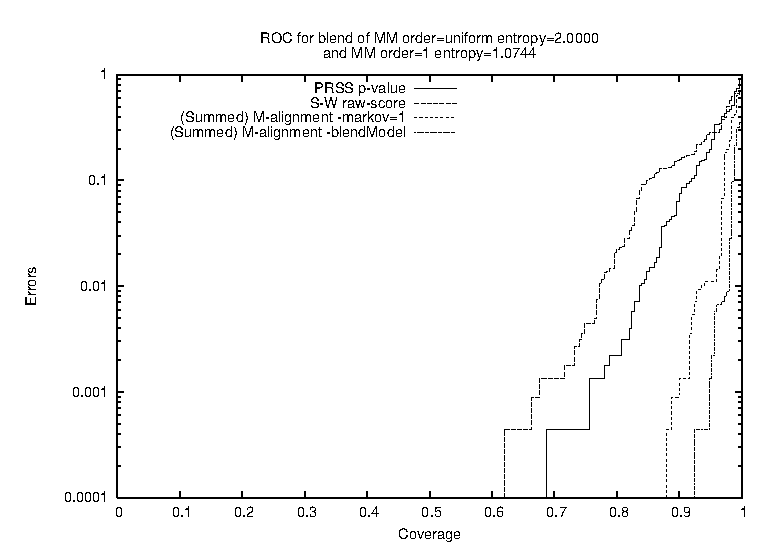
\epsfig{file=roc_blend.eps, width=\plotwidth}
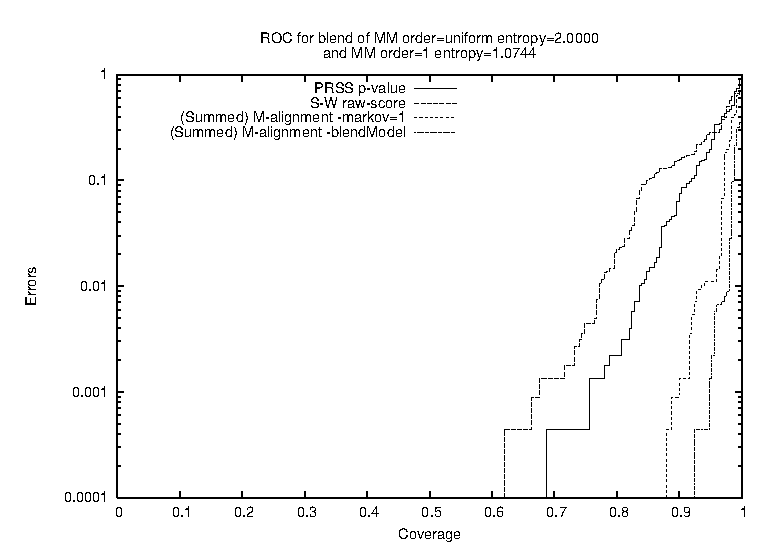
\includegraphics{roc_blend}
\caption{\label{fig:roc_blend}ROC for a blended model}
\end{figure}

%\normalsize
\end{document}

